\chapter{Arquitetura funcional}

O diagrama da Figura \ref{fig:arq_funcional} expôe uma representação da arquitetura funcional do sistema. As setas representam o sentido dos fluxos de dados entre cada função do sistema. 

``Comunicação com o computador'' envolve a UART (física e driver), e o protocolo de comunicação do sistema. Esta função é utilizada para a comunicação com o simulador de elevador, que é executada em um computador. ``Recebe entrada dos botões'' recebe requisições dos botões internos e externos de andares, feitas pelos usuários do elevador. A função ``Controla luzes dos botões'' é responsável por ligar ou desligar as luzes dos botões de acordo com as requisições recebidas dos usuários e de acordo com o movimento do elevador. ``Enfileira requisições'' é responsável por organizar as requisições de botões na ordem em que devem ser atendidas. ``Controla movimento das portas'' efetua a abertura e fechamento das portas, de acordo com a lógica de funcionamento do elevador. ``Controla movimento do elevador'' é responsável por fazer o elevador subir ou descer para atender às requisições enfileiradas.

\begin{figure}[h]
    \centering
    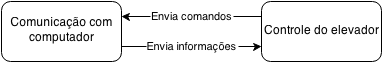
\includegraphics[width=0.8\columnwidth]{./figures/arq_funcional.png}
    \caption{Diagrama da arquitetura funcional do sistema.}
    \label{fig:arq_funcional}
\end{figure}

\section{Alocação das funções em Hardware e Software}

\begin{table}[h!]
\caption{Alocação das funções em Hardware e Software.}
\centering
\begin{tabular}{|c|c|c|}
\hline
\textbf{Bloco} &\textbf{Hardware} & \textbf{Software} \\ \hline \hline
Comunicação com o computador & X & X \\
Recebe entrada dos botões & - & X \\
Controla luzes dos botões & - & X \\
Enfileira requisições & - & X \\
Controla movimento das portas & - & X \\
Controla movimento do elevador & - & X \\
\hline
\end{tabular}
\label{tab:publicacao}
\end{table}

A função de comunicação com o computador constitui-se tanto de hardware quanto de software. A parte de hardware está relacionada ao periférico UART0 do Kit LPC1768. O software relaciona-se ao driver desenvolvido para inicializar e utilizar este periférico, além do protocolo de comunicação do sistema.

O restante das funções é constituida apenas de software, pois controlam a lógica de operação do sistema, não fazendo diretamente o uso de periféricos.





